\documentclass[xcolor=table]{beamer}

\usepackage{graphbox}       % For centre alignment of graphics
\usepackage{textcomp}       % Text companion fonts
\usepackage{tikz}

% PGF and TikZ definitions for this paper

% TikZ library imports
\usetikzlibrary{positioning}        % Anchor placement support
\usetikzlibrary{calc}               % Coordinate calculations
\usetikzlibrary{shapes.geometric}   % cylinder
\usetikzlibrary{shapes.arrows}      % arrow shapes
\usetikzlibrary{shapes.multipart}
\usetikzlibrary{shapes.symbols}
\usetikzlibrary{fit}                % Fitting outline to shape
\usetikzlibrary{arrows}
\usetikzlibrary{arrows.meta}
\usetikzlibrary{shadows}
\usetikzlibrary{spy}


% Define our colours
\colorlet{normal colour}{green!60!blue!20}  % Normal coloured filled areas
\colorlet{accent colour}{orange!25}         % Accented filled areas
\colorlet{background colour}{black!10}      % Background groups
\colorlet{data colour}{black!50}            % Data flow
\colorlet{trigger colour}{black!80}         % Trigger lines
\colorlet{control colour}{blue!50}          % Other lines etc


% Common TikZ definitions
\tikzset{
    % This seems a reasonably comfortable arrow shape
    >=stealth,
%
    % Define a set of styles
    % First some fills
    background fill/.style={fill=background colour},
    highlight fill/.style={fill=normal colour},
    accent fill/.style={fill=accent colour},
    % Next some lines
    bus/.style={draw, color=data colour, text=black, line width=0.6mm, ->},
    control/.style={color=control colour, text=black, very thick, ->},
%
    % Used for creating an exact fit to an existing list of objects
    tight fit/.style={fit=#1, inner sep=0, line width=0},
    % We almost always want centre aligned node text
    every node/.style={align=center},
%
    box/.style={
        draw, rectangle, very thick, highlight fill,
        minimum width=1.5cm, minimum height=1.1cm},
    small box/.style={
        draw, rectangle, thick, highlight fill},
    component/.style={
        draw, rectangle, thick, accent fill,
        minimum width=11mm, minimum height=8mm},
    buffer/.style={
        regular polygon, regular polygon sides=3, anchor=center,
        accent fill, thick, draw},
    generate/.style={
        background fill, thin, draw=gray,
        copy shadow={
            shadow xshift=1ex, shadow yshift=-1ex}},
%
    small label/.style={anchor=south west, inner sep=2pt, font=\small},
%
    trigger line/.style={thin, trigger colour},
    trigger/.style={
        trigger line, >={Triangle[open, scale=1.2]}, shorten >=-5pt, ->},
    trigger dot/.style={fill, circle, inner sep=1pt, line width=-1pt},
    mul/.style={
        draw=black, circle, thick, highlight fill, inner sep=0.5ex},
%
    inline text/.style={
        baseline=(current bounding box.base),
        every node/.append style={anchor=base, font=\scriptsize},},
%
    pics/buffer/.style args={#1/#2}{
        code={
            \draw [thick, -, black] (0.5mm,-2mm) -- (0.5mm,2mm);
            \draw [thick, -, black] (-0.5mm,-2mm) -- (-0.5mm,2mm);
            \node at (0,2mm) [
                rotated anchor=-90, font=\scriptsize, inner sep=0.2em] {#1}
            node at (0,-2mm) [
                rotated anchor=90, font=\scriptsize, inner sep=0.2em] {#2};}},
%
% A helper for drawing ADC and DAC symbols
    adc-dac/.style={
        draw, thick, accent fill, signal, signal to=#1,
        minimum height=8mm, signal pointer angle=120
    },
}


% New tikz key definitions to control behaviour of \multipath.
\tikzset{
    % Default colour for multipath background
    multipath background/.initial=white,
    multipath margin/.initial=0.3mm,
}

% Draws multiple paths with an outline on each path.  Call with path options as
% first optional argument and with a list of paths as the second argument.
\newcommand{\multipath}[2][]{
    \begin{scope}[#1]
        % Pick up multipath margin and background definitions
        \newcommand{\margin}{\pgfkeysvalueof{/tikz/multipath margin}}
        \newcommand{\background}{\pgfkeysvalueof{/tikz/multipath background}}

        % Draw a white background a bit larger than the programmed line
        % thickness.  We turn off any arrows and shorten the line a trifle to
        % avoid any erosion of the endpoints.
        \begin{scope}[
            line width=\pgflinewidth+\margin, color=\background,
            shorten >=\margin, shorten <=\margin, -]
        #2
        \end{scope}

        % Now draw the target path with its original options.
        #2
    \end{scope}
}

% Special coordinates along edge of box
\newcommand{\northcoord}[3]{
    \coordinate (#1 #2) at ($(#1.north west)!#3!(#1.north east)$)}
\newcommand{\eastcoord}[3]{
    \coordinate (#1 #2) at ($(#1.south east)!#3!(#1.north east)$)}
\newcommand{\southcoord}[3]{
    \coordinate (#1 #2) at ($(#1.south west)!#3!(#1.south east)$)}
\newcommand{\westcoord}[3]{
    \coordinate (#1 #2) at ($(#1.south west)!#3!(#1.north west)$)}


% Trick for reusing last coordinate
\makeatletter
\newcommand\lastcoord{\the\tikz@lastxsaved,\the\tikz@lastysaved}
\makeatother


% It's convenient to have a background layer
\pgfdeclarelayer{background}
\pgfsetlayers{background,main}


% Useful for inline boxes
\newcommand\smallbox[2][small box]{\tikz [inline text] \node [#1] {#2};}


% ------------------------------------------------------------------------------
% This frightening looking code is used to compute an anchor that rotates with
% the entire picture.  This is useful when anchoring a node in a pic that itself
% will be rotated.
%   Some really tricky code taken from stack overflow question here:
%
%   https://tex.stackexchange.com/questions/128565/
%       how-to-allow-labels-anchors-in-tikz-to-be-affected-by-
%       rotations-without-rotatin

% \pgfmath@smuggleone
%
% Smuggle a macro outside a group.
%
% Changed by TT: Speedup by insisting, that smuggleone is directly
% followed by \endgroup
%
\makeatletter
\def\pgfmath@smuggleone#1\endgroup{%
  \expandafter\endgroup\expandafter\def\expandafter#1\expandafter{#1}}

\let\pgfmathsmuggle=\pgfmath@smuggleone
\makeatother

\tikzset{
    rotated anchor/.code=%
        \begingroup
            \pgfcoordinate{qrr@origin}{\pgfpointorigin}%
            \pgfcoordinate{qrr@direct}{\pgfpointpolarxy{#1}{1}}%
            \pgftransformreset
            \pgfmathanglebetweenpoints{%
                \pgfpointanchor{qrr@origin}{center}}{%
                    \pgfpointanchor{qrr@direct}{center}}%
            \pgfmathsmuggle\pgfmathresult
        \endgroup
    \tikzset{anchor/.expanded=\pgfmathresult}%
}

% ------------------------------------------------------------------------------

% vim: set filetype=tex:


\setbeamertemplate{navigation symbols}{}

\hyphenpenalty 4000 \sloppy


\title{%
    High speed Tune Measurement using \\
    Phase Following on Multi-Bunch Feedback}
\author{Michael Abbott}
\institute{Diamond Light Source}
\date{Tuesday 4\textsuperscript{th} June 2019}


\begin{document}

\frame{\titlepage}


% ------------------------------------------------------------------------------
%
\begin{frame}{TMBF and LMBF at Diamond Light Source}

\tikzset{
    actuator/.style={circle, inner sep=1pt, highlight fill, draw=black}}

\begin{centering}
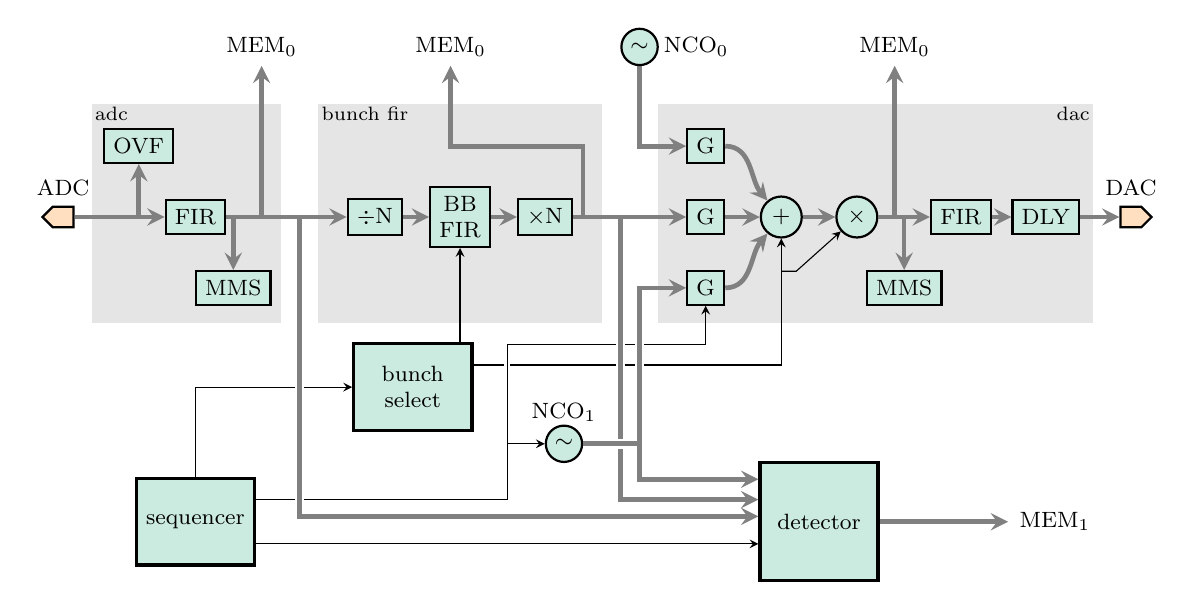
\begin{tikzpicture}[
    adc-dac/.style={
        draw, single arrow, thick, accent fill,
        single arrow head extend=0pt, shape border rotate=#1},
    area label/.style={anchor=north west, font=\scriptsize, inner sep=1pt},
    mul/.style={
        draw=black, circle, thick, highlight fill, inner sep=0.5ex},
    every node/.append style={font=\footnotesize},
    control mux/.style={
        small box, accent fill, label={[font=\tiny]above:MUX}, font=\tiny},
    x=12mm, y=9mm
    ]

    \path [background fill] (0.3,1.6)
        node [area label] {adc} rectangle ++(2,-3.1);
    \path [background fill] (2.7,1.6)
        node [area label] {bunch fir} rectangle ++(3.0,-3.1);
    \path [background fill] (6.3,1.6) rectangle ++(4.6,-3.1)
        ++(0,3.1) node [area label, anchor=north east] {dac};

    \path
        (0,0) node [adc-dac=180, label={ADC}] (adc in) {}
        +(0.8,1) node [small box] (adc ovf) {OVF}
        ++(1.4,0) node [small box] (adc fir) {FIR}
        +(0.4,-1) node [small box] (adc mms) {MMS}
        +(0.7,2.4) node (adc mem) {MEM\textsubscript{0}}
        ++(1.9,0) node [small box] (decimate) {$\div$N}
        ++(0.9,0) node [small box] (bb fir) {BB\\FIR}
        ++(0.9,0) node [small box] (interpolate) {$\times$N}
        +(-1,2.4) node (fir mem) {MEM\textsubscript{0}}
        ++(1.7,0) node [small box] (fir gain) {G}
        +(0,1) node [small box] (nco0 gain) {G}
        +(0,-1) node [small box] (nco1 gain) {G}
        ++(0.8,0) node [mul] (sum) {$+$}
        ++(0.8,0) node [mul] (product) {$\times$}
        +(0.5,-1) node [small box] (dac mms) {MMS}
        +(0.4,2.4) node (dac mem) {MEM\textsubscript{0}}
        ++(1.1,0) node [small box] (dac fir) {FIR}
        ++(0.9,0) node [small box] (delay) {DLY}
        ++(0.9,0) node [adc-dac, label={DAC}] (dac out) {};

    \node [box] at (1.4,-4.3) (sequencer) {sequencer};
    \path (bb fir) ++(-0.5,-2.4) node [box] (bunch) {bunch\\select};
    \node [box, minimum height=15mm] at (8,-4.3) (detector) {detector};
    \path (nco1 gain) ++(-1.5,-2.2)
        node [mul,
            label={[inner sep=1pt]above:NCO\textsubscript{1}}] (nco1) {$\sim$};

    \draw [bus] (adc in) -- (adc fir);
    \draw [bus] (adc in) -| (adc ovf);
    \draw [bus] (adc fir) -| (adc mms);
    \draw [bus] (adc fir) -| (adc mem);
    \draw [bus] (adc fir) -- (decimate);

    \draw [bus] (decimate) -- (bb fir);
    \draw [bus] (bb fir) -- (interpolate);
    \draw [bus] (interpolate) -- (fir gain);
    \draw [bus] (interpolate) ++(0.4,0) -- ++(0,1) -| (fir mem);
    \draw [bus] (fir gain) -- (sum);
    \draw [bus] (nco0 gain) to [out=0, in=130] (sum);
    \draw [bus] (nco1 gain) to [out=0, in=-130] (sum);
    \draw [bus] (sum) -- (product);
    \draw [bus] (product) -- (dac fir);
    \draw [bus] (product) -| (dac mms);
    \draw [bus] (product) -| (dac mem);
    \draw [bus] (dac fir) -- (delay);
    \draw [bus] (delay) -- (dac out);

    \draw [bus, <-] (nco0 gain) -- ++(-0.7,0) -- ++(0,1.4)
        node [mul, label={[inner sep=1pt]right:NCO\textsubscript{0}}] {$\sim$};

    \draw [thin, ->] (sequencer) |- (bunch);
    \draw [thin, ->] (bunch.north-|bb fir) -- (bb fir);
    \draw [thin, <-] (product) -- ++(-130:1) -- (\lastcoord-|sum);
    \draw [thin, ->] (bunch.20) -| (sum);
    \draw [thin, ->] (sequencer.-20) -- (\lastcoord-|detector.west);
    \draw [thin, ->] (sequencer.20) -| ($(nco1)+(-0.6,0)$)
        coordinate (nco1 control) -- (nco1);
    \multipath [thin] {\draw (nco1 control) -- ++(0,1.4);}
    \draw [thin, ->] (nco1 control) -- ++(0,1.4) -| (nco1 gain);

    \multipath [bus] {\draw (interpolate) ++(0.8,0) |- (detector.160);}
    \multipath [bus] {\draw (adc fir) ++(1.1,0) |- (detector.175);}
    \multipath [bus, -] {
        \draw (nco1) -- ++(0.8,0) -- (\lastcoord|-nco1 gain);
        \draw (nco1) -- ++(0.8,0) -- (\lastcoord|-detector.145);
    }
    \draw [bus] (nco1) ++(0.8,0) |- (nco1 gain);
    \draw [bus] (nco1) ++(0.8,0) |- (detector.145);

    \draw [bus] (detector) -- ++(2,0)
        node [anchor=west] {MEM\textsubscript{1}};

\end{tikzpicture}

% vim: filetype=tex:

\end{centering}

\bigskip
\smallbox[actuator]{B} EBPM pickup;
\smallbox[actuator]{C} Longitudinal cavity;
\smallbox[actuator]{S} Transverse striplines.

\end{frame}


% ------------------------------------------------------------------------------
%
\begin{frame}{MBF Signal Processing Chain}

\begin{tikzpicture}[
    switch/.style={
        small box, inner sep=1pt,
        node contents={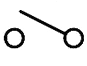
\includegraphics[width=1.5em]{switch.png}},
    },
    x=15mm, y=15mm]

\path
    (0,1.5) node (adc) [adc-dac=west] {ADC}
    ++(2,0) node [box] (fir) {Feedback\\FIR}
    (5,0) node [mul] (dac sum) {$+$}
    ++(1.5,0) node [adc-dac=east] (dac) {DAC}

    (2.4,0.5) node [small box] (nco1) {NCO\textsubscript1}
    ++(0,-1)
    +(1ex,-1ex) node [small box] {\phantom{NCO\textsubscript2}}
    +(0,0) node [small box] (nco2) {NCO\textsubscript2}
    ++(0,-1)
    +(1ex,-1ex) node [small box] {\phantom{NCO\textsubscript3}}
    +(0,0) node [small box] (nco3) {NCO\textsubscript3}

    (0.5,-0.5)
    node [box] (sweep) {Sweep}

    (0.5,-1.5)
    node [box] (tune pll) {Tune\\Pll}

    (4,1.5) node (fir enable) [switch]
    ++(0,-1) node (nco1 enable) [switch]
    ++(0,-1) node (nco2 enable) [switch]
    ++(0,-1) node (nco3 enable) [switch]

    (3.45,-2.6) node [box] (enables) {Bunch\\Enables}

    (4.9,-1.4) node [anchor=north west] {\parbox{32mm}{
        \scriptsize
        Key:
        \begin{enumerate}
            \item[\smallbox{NCO}] Numerically Controlled Oscillator.
            \item[{\tikz [inline text] \node [switch];}] Output enable.
        \end{enumerate}
    }};

\begin{pgfonlayer}{background}
    \node [fill=background colour, fit=(tune pll) (nco3 enable)] (new) {};
\end{pgfonlayer}
\path (new.south west) node [anchor=north west, color=black!50] {New};

\draw [->] (enables.north -| fir enable)
    +(-0.7,0) -- ($(fir enable)-0.7*(1,1)$) -- (fir enable);
\draw [->] (enables.north -| nco1 enable)
    +(-0.6,0) -- ($(nco1 enable)-0.6*(1,1)$) -- (nco1 enable);
\draw [->] (enables.north -| nco2 enable)
    +(-0.5,0) -- ($(nco2 enable)-0.5*(1,1)$) -- (nco2 enable);
\draw [->] (enables.north -| nco3 enable)
    +(-0.4,0) -- ($(nco3 enable)-0.4*(1,1)$) -- (nco3 enable);

\draw [bus] (adc) -- (fir);
\draw [bus]
    (sweep.east |- nco1) node [anchor=east] {f\textsubscript1} -- (nco1);
\draw [bus] (sweep) -- (nco2)
    node [midway, inner sep=1pt, label=above:f\textsubscript2] {};
\draw [bus] (tune pll) -- (nco3)
    node [midway, inner sep=1pt, label=above:f\textsubscript3] {};

\draw [bus] (fir) -- (fir enable);
\multipath [bus] {
    \draw (nco1) -- (nco1 enable);
    \draw (nco2) -- (nco2 enable);}
\multipath [bus, multipath background=background colour] {
    \draw (nco3) -- (nco3 enable);}

\draw [bus] (fir enable) -- +(0.5,0) -- (dac sum);
\draw [bus] (nco1 enable) -- +(0.5,0) -- (dac sum);
\draw [bus] (nco2 enable) -- +(0.5,0) -- (dac sum);
\draw [bus] (nco3 enable) -- +(0.5,0) -- (dac sum);

\draw [bus] (dac sum) -- (dac);

\end{tikzpicture}

% vim: filetype=tex:


\end{frame}


% ------------------------------------------------------------------------------
%
\begin{frame}{Measuring Beam Frequency Response}

\begin{centering}
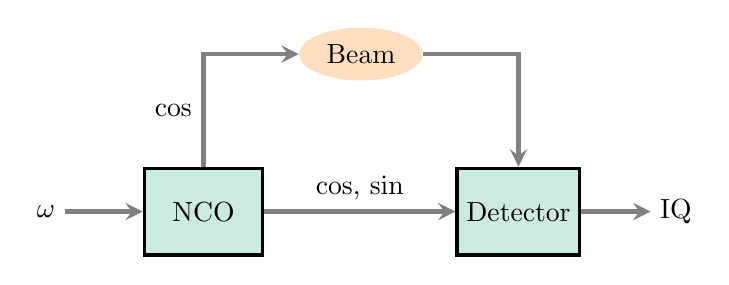
\begin{tikzpicture}[x=20mm, y=20mm]

\path
    (0,0) node [box] (nco) {NCO}
    +(-1,0) node (f) {$\omega$}
    (1,1) node [accent fill, ellipse] (beam) {Beam}
    (2,0) node [box] (detector) {Detector}
    +(1,0) node (iq) {IQ};

\draw [bus] (f) -- (nco);
\draw [bus] (nco) |- (beam) node [pos=0.25, left] {cos};
\draw [bus] (beam) -| (detector);
\draw [bus] (nco) -- (detector) node [midway, above] {cos, sin};
\draw [bus] (detector) -- (iq);

\end{tikzpicture}

% vim: filetype=tex:

\end{centering}

\bigskip

By exciting the beam at a selected frequency $f$ and measuring the response of
the beam at that frequency, we compute the \emph{transfer function} of the
machine at the selected frequency.

\begin{equation*}
    R(f) = \sum_{t\in\text{dwell}} e^{2\pi i f t} x_t
\end{equation*}

This can be expressed as phase and magnitude, or equivalently as a
complex number, or in digital processing terms as a pair (I,Q).

\end{frame}


% ------------------------------------------------------------------------------
%
\begin{frame}{Implementation of Detector}

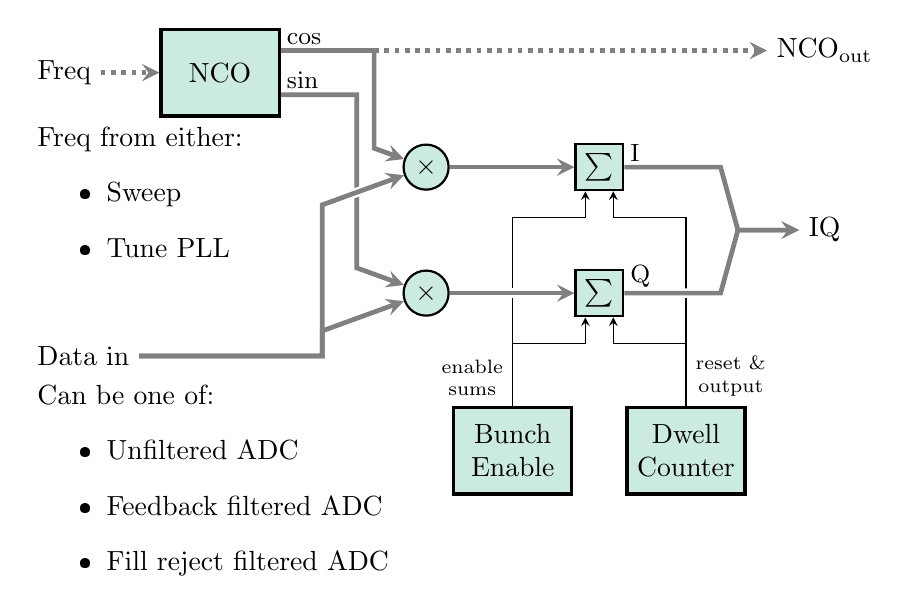
\begin{tikzpicture}[x=22mm, y=8mm]

\path
    +(0,-2) node (data in) [anchor=west] {Data in}
    +(0,2.5) node (f in) [anchor=west] {Freq}
    (2.3,0)
    +(0,1) node [mul] (cos prod) {$\times$}
    +(0,-1) node [mul] (sin prod) {$\times$}
    +(0.5,-3.5) node [box] (bunch) {Bunch\\Enable}
    +(1.5,-3.5) node [box] (dwell) {Dwell\\Counter}
    ++(1,0)
    +(0,1) node [small box] (cos sum) {$\sum$}
    +(0,-1) node [small box] (sin sum) {$\sum$}
    ++(0.8,0) coordinate (gather iq)
    ++(0.5,0) node (iq out) {IQ};

\path (f in) +(0.9,0) node [box] (nco) {NCO}
    (nco.east) +(0,0.35) coordinate (cos in)
    (nco.east) +(0,-0.35) coordinate (sin in)
    (cos in -| iq out) node (cos out) {NCO\textsubscript{out}};

\path [
    anchor=north west, text width=50mm, every node/.style=, align=left]
(data in.south west) node {
    Can be one of:
    \begin{itemize}
    \item Unfiltered ADC
    \item Feedback filtered ADC
    \item Fill reject filtered ADC
    \end{itemize}
}
(data in.west |- nco.south) node {
    Freq from either:
    \begin{itemize}
    \item Sweep
    \item Tune PLL
    \end{itemize}
};

\path (cos sum.east) [small label] node {I};
\path (sin sum.east) [small label] node {Q};

\draw [->] (bunch) -- ($(bunch |- cos sum)-(0,0.8)$) -| (cos sum.-120);
\draw [->] (bunch) -- ($(bunch |- sin sum)-(0,0.8)$) -| (sin sum.-120);
\node at (bunch.north)
    [anchor=south east, font=\scriptsize] {enable\\sums};
\draw [->] (dwell) -- ($(dwell |- cos sum)-(0,0.8)$) -| (cos sum.-60);
\draw [->] (dwell) -- ($(dwell |- sin sum)-(0,0.8)$) -| (sin sum.-60);
\node at (dwell.north)
    [anchor=south west, font=\scriptsize] {reset \&\\output};

\path (cos in) [small label] node {cos};
\path (sin in) [small label] node {sin};

\path [bus] (cos in) -| ($(cos prod)-0.3*(1,-1)$) -- (cos prod);
\path [bus] (sin in) -| ($(sin prod)-0.4*(1,-1)$) -- (sin prod);
\multipath [bus] { \draw (data in) -| ($(cos prod)-0.6*(1,1)$) -- (cos prod); }
\path [bus] (data in) -| ($(sin prod)-0.6*(1,1)$) -- (sin prod);

\draw [bus] (cos prod) -- (cos sum);
\multipath [bus] {
    \draw (sin prod) -- (sin sum);
    \draw (cos sum) -- ++(0.7,0) -- (gather iq) -- (iq out);
    \draw (sin sum) -- ++(0.7,0) -- (gather iq) -- (iq out);}
\draw [bus, dotted] (f in) -- (nco);
\draw [bus, dotted] (cos in -| cos prod) +(-0.3,0) -- (cos out);

\end{tikzpicture}

% vim: filetype=tex:


\end{frame}


% ------------------------------------------------------------------------------
%
\begin{frame}{Typical Tune Sweep Response}

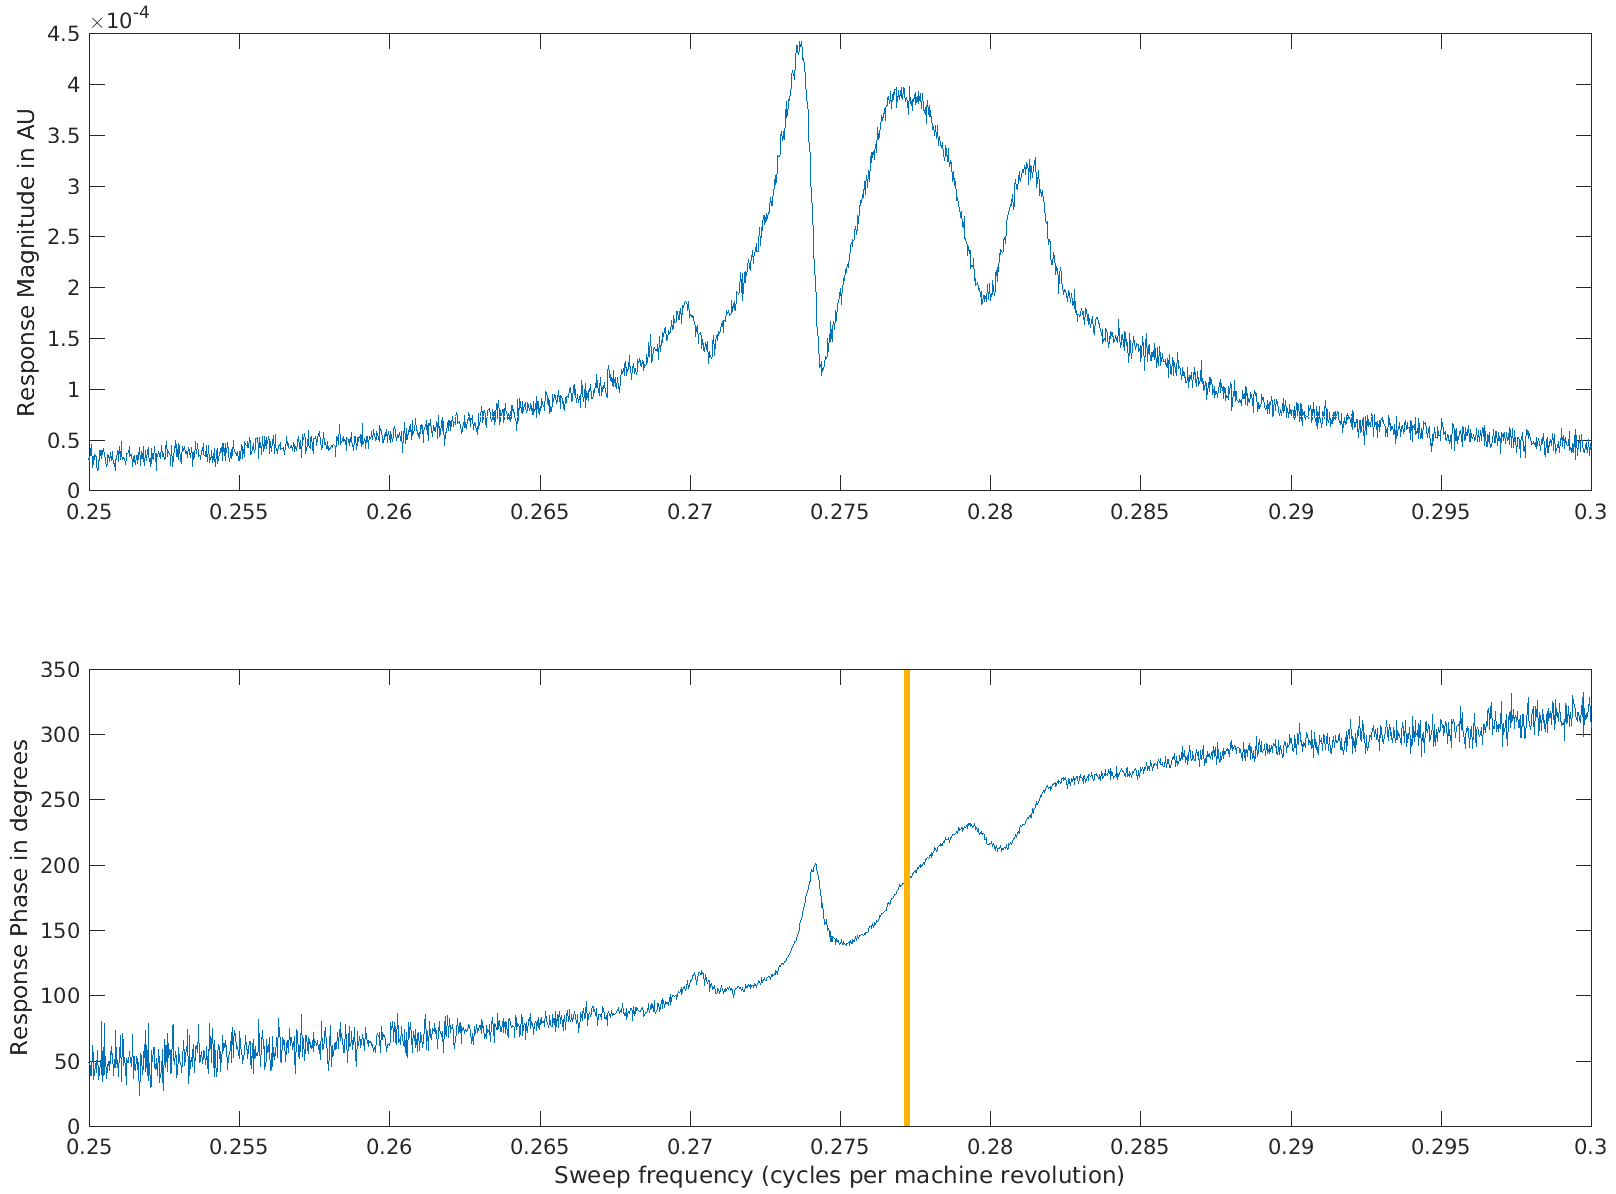
\includegraphics[width=\linewidth]{tune-sweep-complex.png}

\end{frame}


% ------------------------------------------------------------------------------
%
\begin{frame}{Measuring Tune by Tracking Phase}

\begin{itemize}
\item Define desired target phase response (eg, 180\textdegree).
\item Excite selected region of beam with Tune PLL NCO at selected single
    frequency.
\item Measure phase response at this frequency.
\item Use difference between measured and target phase to update frequency (a
    simple PI controller is sufficient).
\item Repeat.
\end{itemize}

This is implemented on the FPGA, and can run at more than 100\,kHz; however most
tune motion seems to be concentrated between $10^2$ and $10^{-2}$\,Hz, and a
sensible rate is around 2\,kHz.

\end{frame}


% ------------------------------------------------------------------------------
%
\begin{frame}{Tune PLL Implementation}

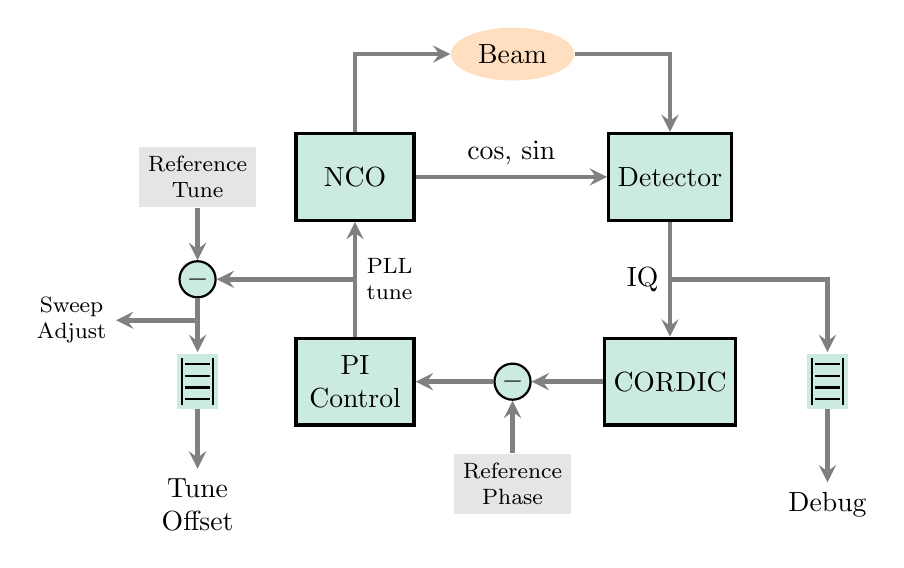
\begin{tikzpicture}[
    queue box/.style={
        highlight fill,
        inner sep=1pt,
        node contents={\includegraphics[width=3ex]{queue.png}}},
    x=20mm, y=26mm]

\tikzset{
    % An attempt to draw a simple queue.  Not all that great, to be honest
    queue/.pic={\scoped [x=2mm,y=1.5mm] {
        \path [highlight fill] (-1.3,-2.3) rectangle (1.3,2.3);
        \draw [thick]
            (-1,-2) -- +(0,4)
            (1,-2) -- +(0,4)
            (-0.8,-1.5) foreach \x in {-1,...,2} { -- +(1.6,0) ++(0,1) };
    }}
}

\path
    (0,0) node [box] (nco) {NCO}
    (1,0.6) node [accent fill, ellipse] (beam) {Beam}
    (2,0) node [box] (detector) {Detector}
    (2,-1) node [box] (cordic) {CORDIC}
    +(1,-0.6) node (debug out) {Debug}
    (1,-1) node [mul, inner sep=1pt] (ref diff) {$-$}
    +(0,-0.5) node [font=\footnotesize, background fill]
        (ref phase) {Reference\\Phase}
    (0,-1) node [box] (control) {PI\\Control}
    +(-1,-0.6) node (tune out) {Tune\\Offset}
    (-1,-0.5) node [mul, inner sep=1pt] (tune diff) {$-$}
    +(0,0.5) node [font=\footnotesize, background fill]
        (ref tune) {Reference\\Tune}
    +(-0.8,-0.2) node [font=\footnotesize] (sweep) {Sweep\\Adjust};

\path
    (cordic) +(1,0) pic [local bounding box=debug queue] {queue}
    (control) +(-1,0) pic [local bounding box=tune queue] {queue};

\draw [bus] (nco) |- (beam);
\draw [bus] (beam) -| (detector);
\draw [bus] (control) -- node [right, font=\footnotesize] {PLL\\tune} (nco);
\draw [bus] (nco) -- node [above] {cos, sin} (detector);
\draw [bus] (detector) -- node [left] {IQ} (cordic);
\draw [bus] (ref phase) -- (ref diff);
\draw [bus] (cordic) -- node [above] {$\measuredangle$} (ref diff);
\draw [bus] (ref diff) -- (control);

\draw [bus] ($(detector)!0.5!(cordic)$) -| (debug queue);
\draw [bus] (debug queue) -- (debug out);

\draw [bus] (ref tune) -- (tune diff);
\draw [bus] (nco |- tune diff) -- (tune diff);
\draw [bus] (tune diff) |- (sweep);
\draw [bus] (tune diff) -- (tune queue);
\draw [bus] (tune queue) -- (tune out);

\end{tikzpicture}

% vim: filetype=tex:


\end{frame}


% ------------------------------------------------------------------------------
%
\begin{frame}{High Resolution Tune Measurement}

\hspace{0.05\linewidth}
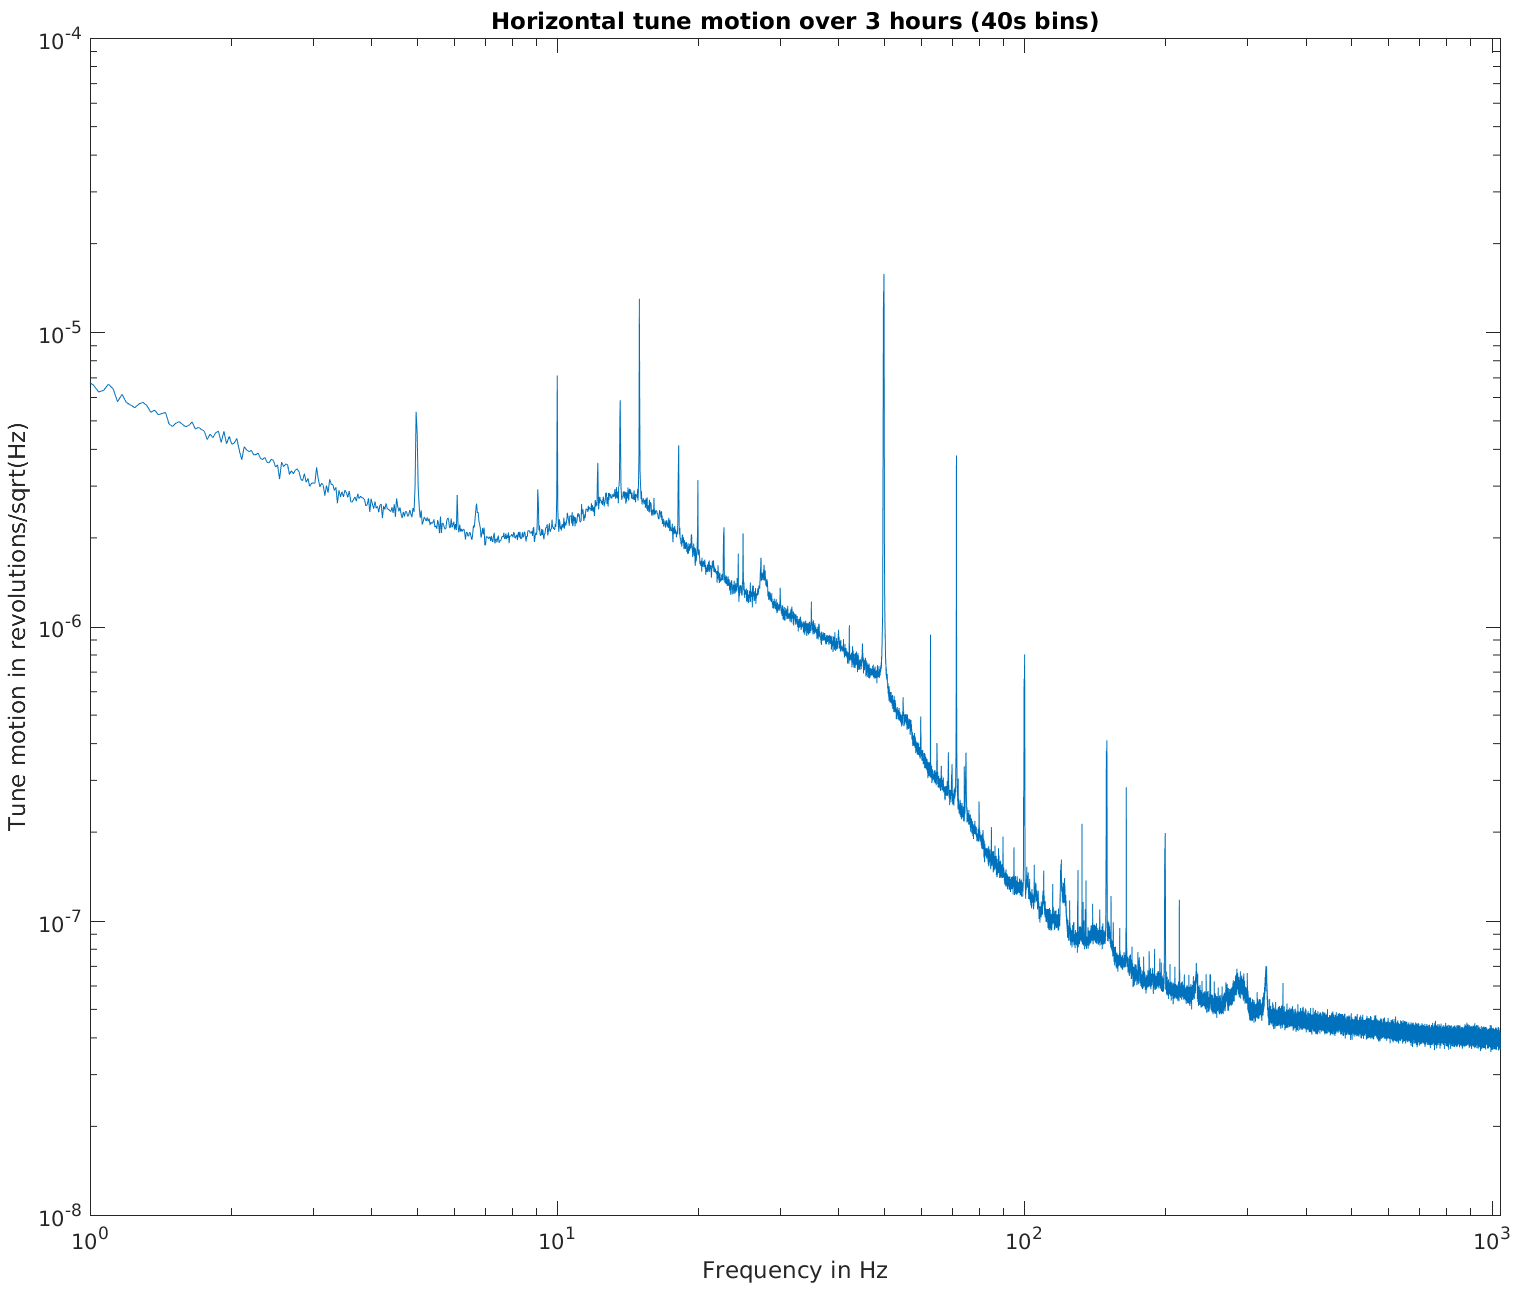
\includegraphics[width=0.9\linewidth]{tune-f40s2-3h.png}

\end{frame}


% ------------------------------------------------------------------------------
%
\begin{frame}{Disturbance to Tune Sweeps}

\begin{tikzpicture}[
    spy using outlines={
        circle, orange, magnification=3, size=50mm, connect spies}]
\node {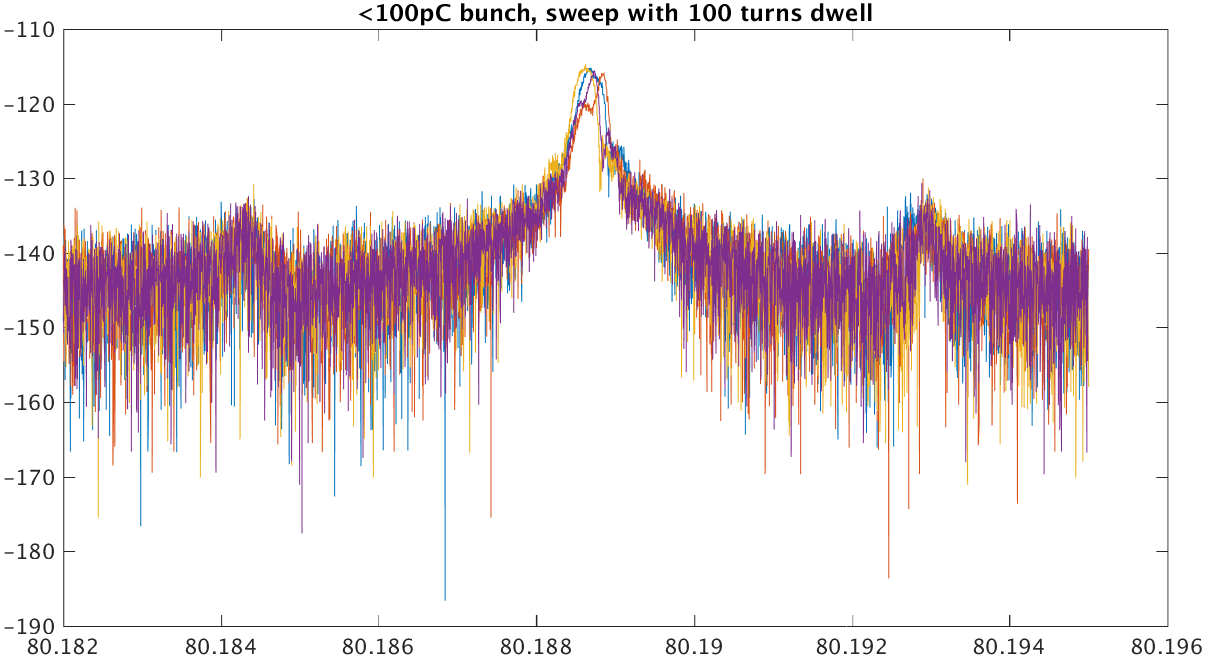
\includegraphics[width=\linewidth]{PLL_small_bunch_sweep1.png}};
\spy on (-0.1,1.8) in node [left] at (5.1,-0.8);
\end{tikzpicture}

\end{frame}


% ------------------------------------------------------------------------------
%
\begin{frame}{Compensating for Tune motion}

\begin{itemize}
\item Tune disturbance is global (all bunches see the same disturbance).
\item Can use PLL to track tune on part of fill.
\item Tune offset then dynamically compensates tune sweep.
\item Can now perform very long sweeps on low current parts of fill.
\end{itemize}

\medskip
\begin{centering}
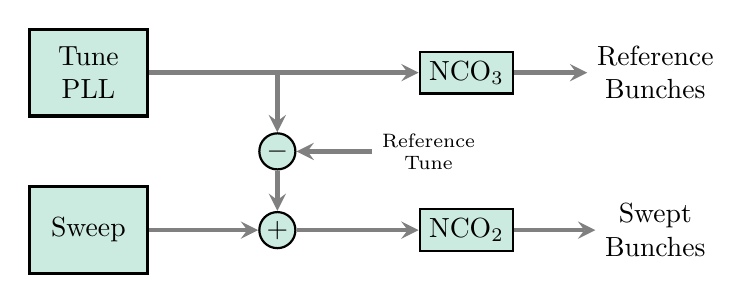
\begin{tikzpicture}[
    x=24mm, y=20mm]

\path
    (0,0) node [box] (tune pll) {Tune\\PLL}
    ++(2,0) node [small box] (nco3) {NCO\textsubscript3}
    ++(1,0) node (reference) {Reference\\Bunches}
    (tune pll)
    ++(1,-0.5) node [mul, inner sep=1pt] (sum pll) {$-$}
    ++(0.8,0) node [font=\scriptsize] (ref tune) {Reference\\Tune}
    (tune pll)
    ++(0,-1) node [box] (sweep) {Sweep}
    ++(1,0) node [mul, inner sep=1pt] (sum sweep) {$+$}
    ++(1,0) node [small box] (nco2) {NCO\textsubscript2}
    ++(1,0) node (target) {Swept\\Bunches};

\draw [bus] (tune pll) -- (nco3);
\draw [bus] (nco3) -- (reference);
\draw [bus] (tune pll) -| (sum pll);
\draw [bus] (ref tune) -- (sum pll);
\draw [bus] (sum pll) -- (sum sweep);
\draw [bus] (sweep) -- (sum sweep);
\draw [bus] (sum sweep) -- (nco2);
\draw [bus] (nco2) -- (target);

\end{tikzpicture}

% vim: filetype=tex:

\end{centering}

\end{frame}


% ------------------------------------------------------------------------------
%
\begin{frame}{Using Bunch Enables}

Machine fill pattern

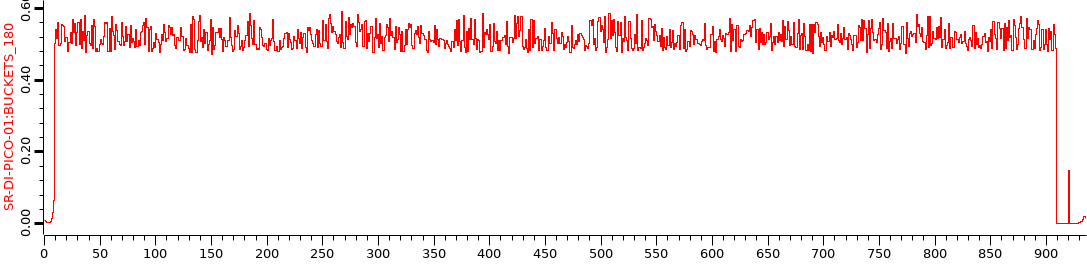
\includegraphics[width=\linewidth]{buckets.png}

\medskip

{
\renewcommand{\arraystretch}{1.5}
\begin{tabular}{>{\raggedright}p{0.5\linewidth}l}
    FIR (feedback) output enable, Tune PLL (NCO\textsubscript3) output enable,
    Tune PLL detector enable. &
    \raisebox{-0.8\height}{
        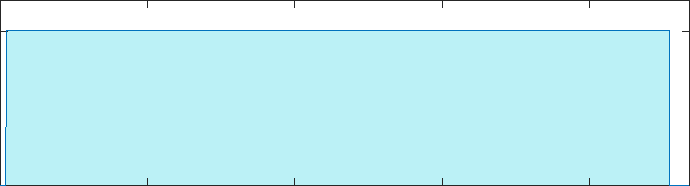
\includegraphics[width=0.4\linewidth]{enable-fill.png}}
    \\
    Sweep (NCO\textsubscript2) output enable, Sweep detector enable. &
    \raisebox{-0.8\height}{
        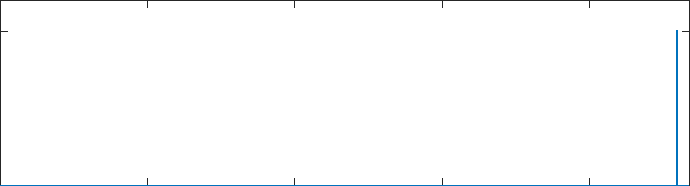
\includegraphics[width=0.4\linewidth]{enable-bunch.png}}
    \\
\end{tabular}
}

\medskip
\footnotesize
With this setup we can do long slow sweeps on the single bunch.

\end{frame}


% ------------------------------------------------------------------------------
%
\begin{frame}{Compensated vs Uncompensated Tune Sweeps}

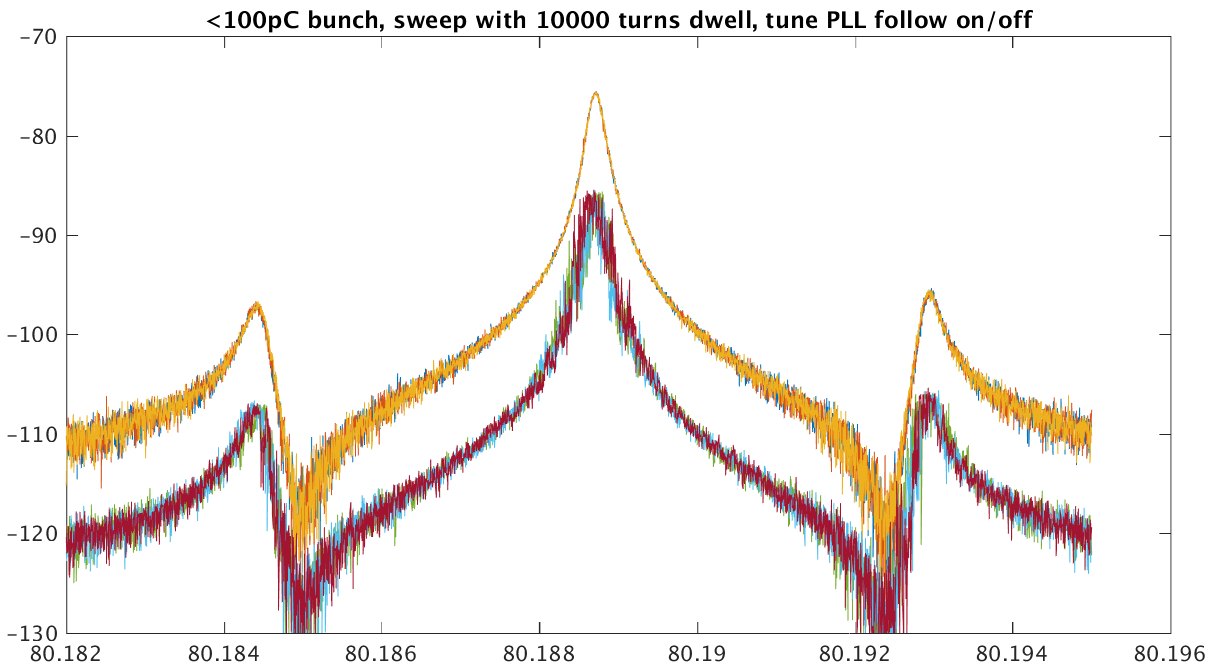
\includegraphics[width=\linewidth]{PLL_small_bunch_sweep4.png}

\end{frame}


% ------------------------------------------------------------------------------
%
\begin{frame}{High resolution slow sweeps}

Slow tune sweeps of 50\,pC single bunch with varying chromaticity.

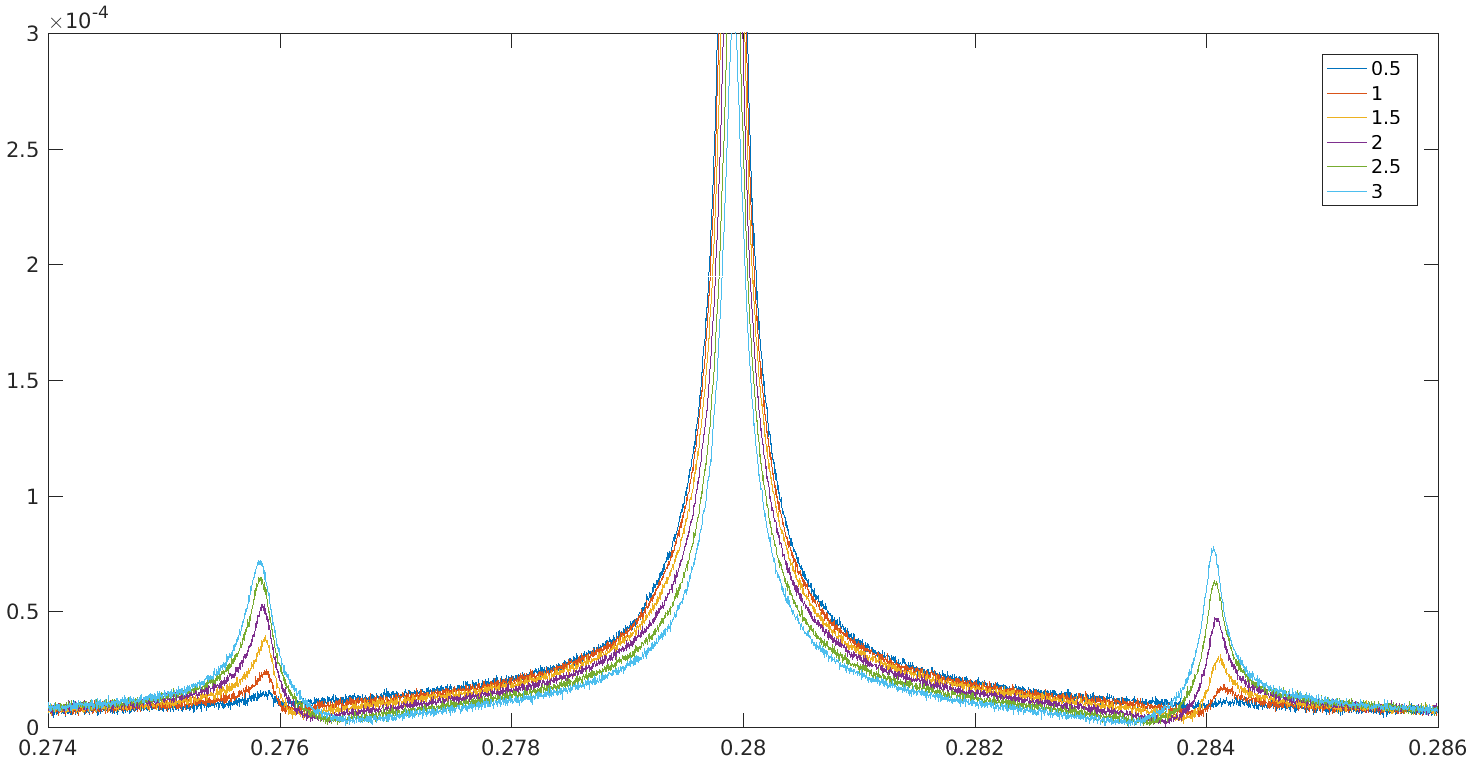
\includegraphics[width=\linewidth]{chro-scan.png}

Now ready to investigate inference of machine chromaticity from high resolution
tune sweep.

\end{frame}


% ------------------------------------------------------------------------------
%
\begin{frame}{Fin}

\vskip0pt plus 1filll
\footnotesize
Some extra slides follow.

\end{frame}


% ------------------------------------------------------------------------------
%
\begin{frame}{Equation for Detector Operation}

\begin{equation*}
    \text{iq}_n = \sum_{t=nDT}^{(n+1)DT-1}
    e^{2\pi i \frac{f_n}{T} t}
        \cdot B(t\mathbin{\text{mod}} T) \cdot x_t
\end{equation*}

\bigskip

\begin{tabular}{>{$}l<{$}l}
n & Number of captured dwell \\
D & Dwell time in turns \\
f_n & Excitation frequency in cycles per machine revolution ($T$ ticks) \\
T & Number of bunches per turn (936 at DLS) \\
t & Time in bunch clock ticks \\
B(b) & Bunch enable for selected bunch $b$ \\
x_t & Sample at time $t$ \\
\end{tabular}

\end{frame}


% ------------------------------------------------------------------------------
%
\begin{frame}{Tune PLL 3 hour Cumulative Sum}

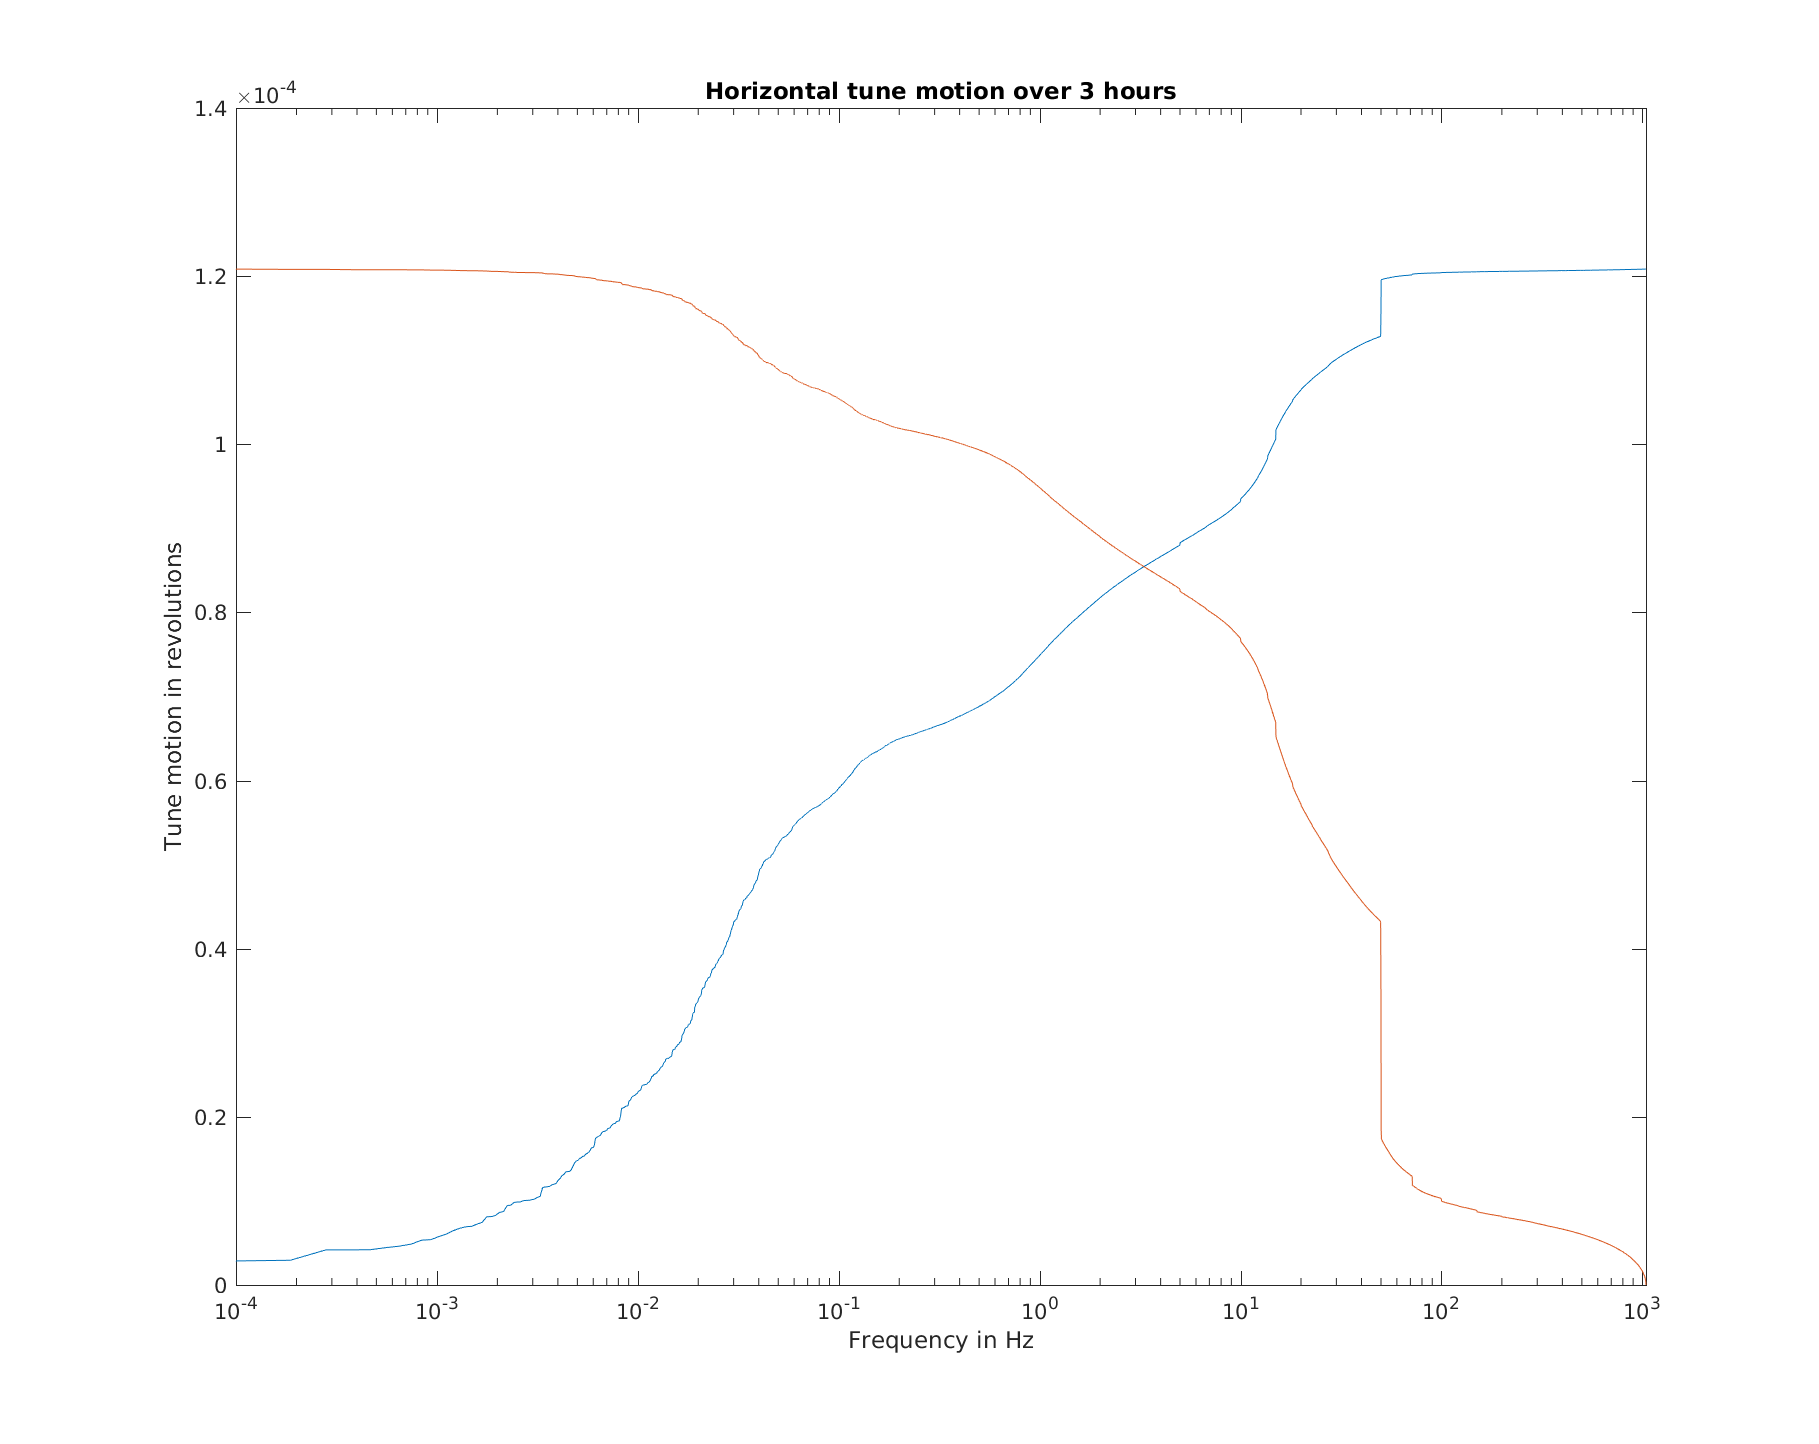
\includegraphics[width=\linewidth]{tune-c-3h.png}

\end{frame}


% ------------------------------------------------------------------------------
%
\begin{frame}{Feedback Residual}

How much noise is the feedback loop introducing?

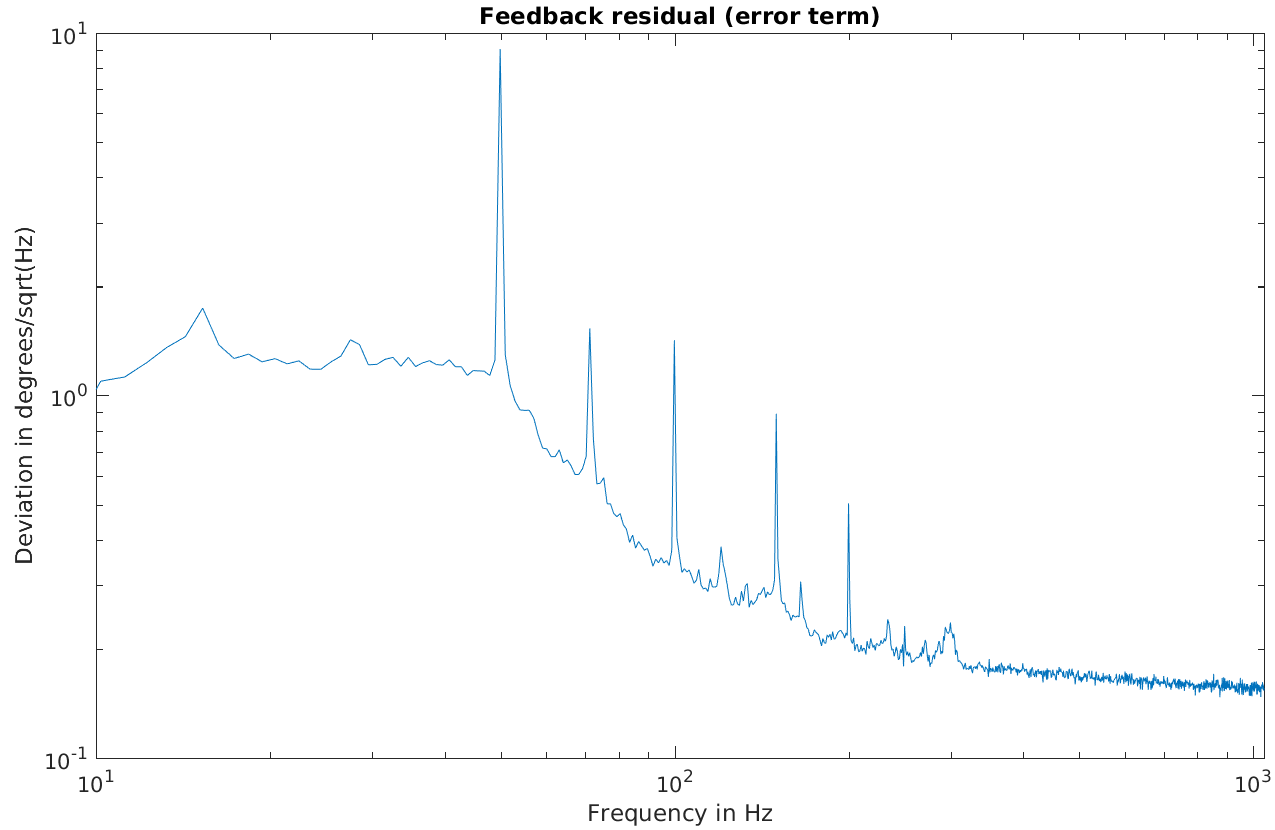
\includegraphics[width=\linewidth]{tune-residual.png}

\end{frame}


\end{document}


% ------------------------------------------------------------------------------
%
\begin{frame}{}

\end{frame}
